\chapter{Interfície d'usuari}
\label{chap:interficie_usuari}

La interfície d'usuari és la part que està més exposada al públic de tot el projecte, ja que serà a través d'on els jugadors de la botifarra viuran les seves experiències i interactuaran amb altres jugadors. Per tal de tenir clar des d'un principi com es volia estructurar es va dissenyar una maqueta de la mateixa abans de començar a treballar. 

\section{Maquetes previes}

\begin{figure}[htbp]
\centering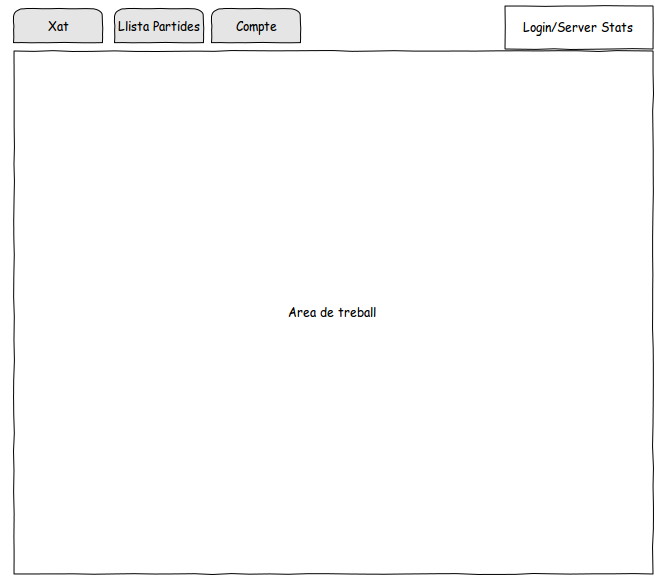
\includegraphics{img/Inici.png}
\caption{Maqueta de la pantalla inicial}
\label{fig:mookup-inici}
\end{figure} 

A la figura \ref{fig:mookup-inici} es pot veure com serà la pantalla inicial. Aquesta s'estructurarà per pestanyes per a que els usuaris puguin accedir a les diferents opcions de la partida. A l'àrea de treball es mostrarà el contingut de les diferents pestanyes. 

\begin{figure}[htbp]
\centering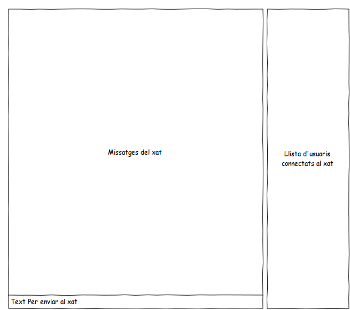
\includegraphics{img/Xat.png}
\caption{Maqueta de la pantalla de Xat}
\label{fig:mookup-xat}
\end{figure} 

A la figura \ref{fig:mookup-xat} es pot veure el contingut que es mostrarà a l'àrea de treball quan la pestanya de xat estigui activa. 

\begin{figure}[htbp]
\centering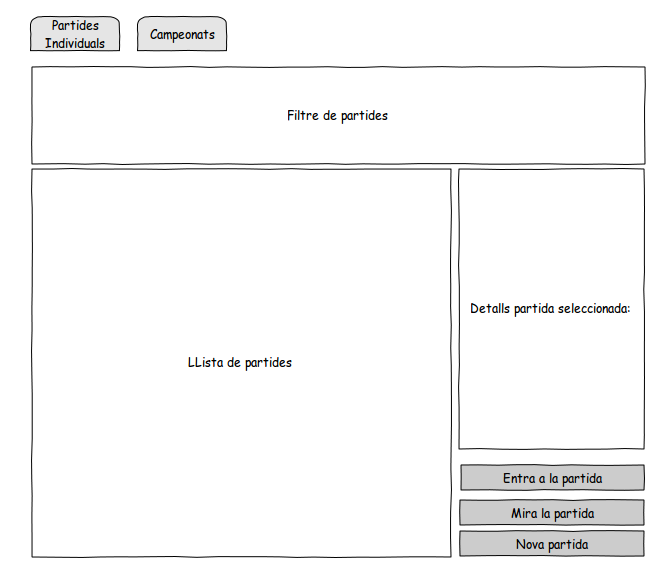
\includegraphics{img/Llista_Partides.png}
\caption{Maqueta del llistat de partides disponibles}
\label{fig:mookup-partides}
\end{figure} 

A la figura \ref{fig:mookup-partides} es pot veure el contingut que es mostrarà a l'àrea de treball quan la pestanya de Llista de partides estigui activa. 

\begin{figure}[htbp]
\centering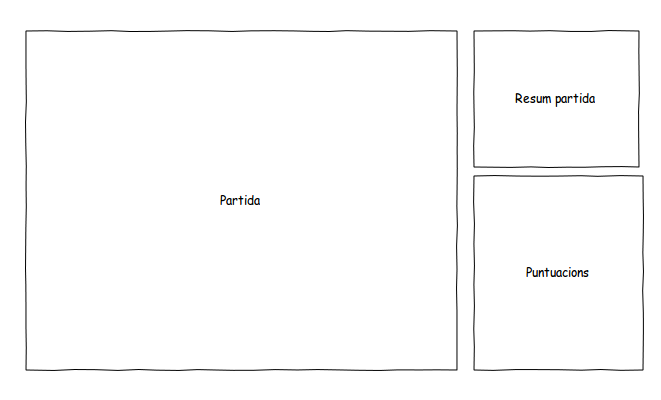
\includegraphics{img/Global_Partida.png}
\caption{Maqueta de la pantalla global de la partida}
\label{fig:mookup-partida}
\end{figure} 

A la figura \ref{fig:mookup-partida} es pot veure el contingut que es mostrarà a l'àrea de treball quan hi hagi una partida en curs. A l'àrea partida serà on els jugadors podran visualitzar el transcurs de la partida i interactuar amb el servidor. Es pot veure en més detall com s'estructura aquesta part en la figura \ref{fig:mookup-detall}.
\begin{figure}[htbp]
\centering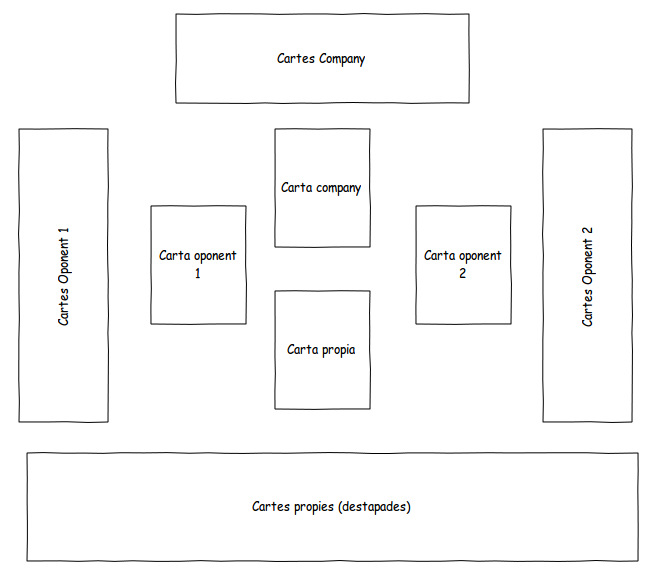
\includegraphics{img/Detall_partida.png}
\caption{Maqueta de la pantalla de detall de la partida}
\label{fig:mookup-detall}
\end{figure} 

\section{Resultat final}

A la figura \ref{fig:real-xat} es pot observar la pantalla que ens mostra l'aplicació després d'identificar-nos. Així al a part equerra podem veure els missatges del xat i a la part dreta la llista d'usuaris que hi ha connectats al servidor. 

\begin{figure}[htbp]
\centering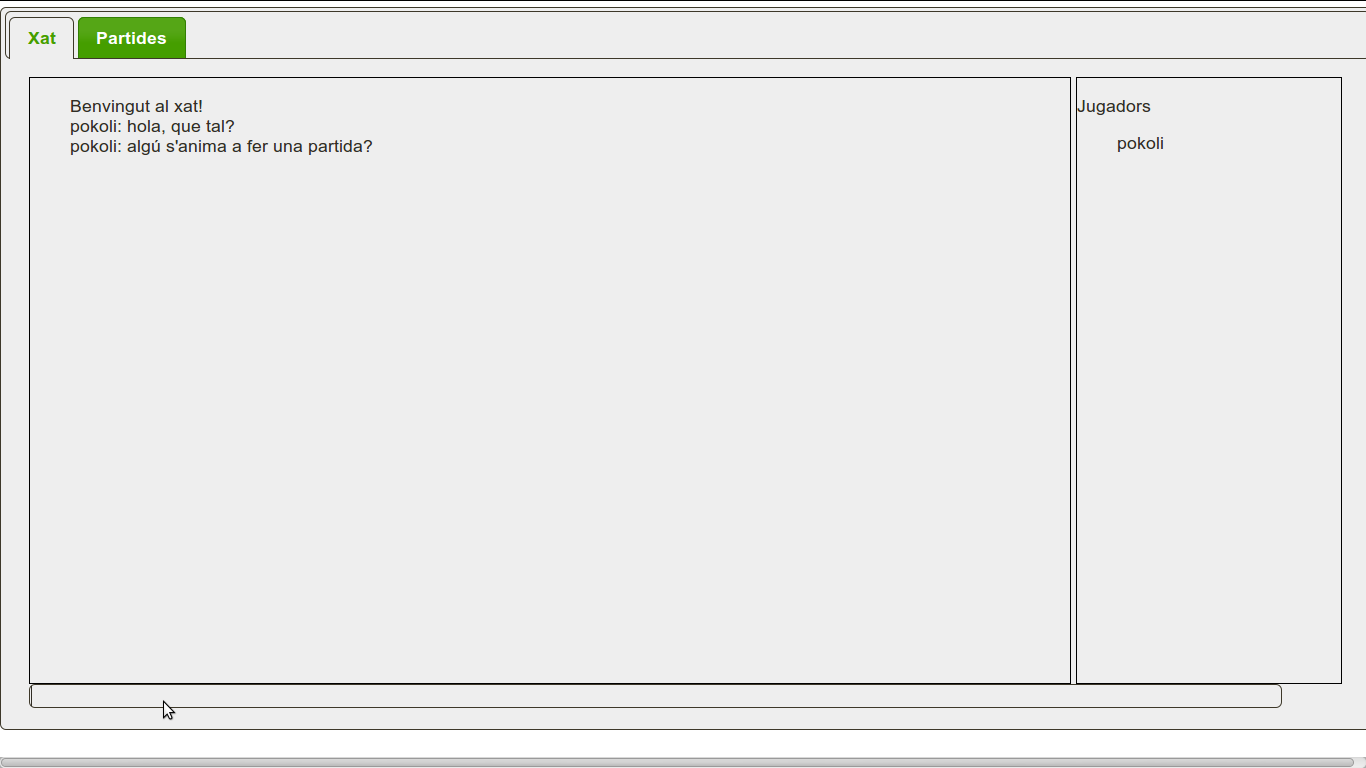
\includegraphics{img/real-xat.png}
\caption{Captura de la pantalla de xat i llista d'usuari.}
\label{fig:real-xat}
\end{figure} 

A la figura \ref{fig:real-partida} es pot veure l'aspecte que té l'aplicació en mitg d'una partida. Així podem veure les nostres cartes, que clicarem per jugar quan sigui el nostre torn, juntament amb les cartes que han jugat els nostres rivals. A la part de la dreta també podem observar les dades generals de la partida, i la puntació de les rondes que s'han jugat fins al moment. 
\begin{figure}[htbp]
\centering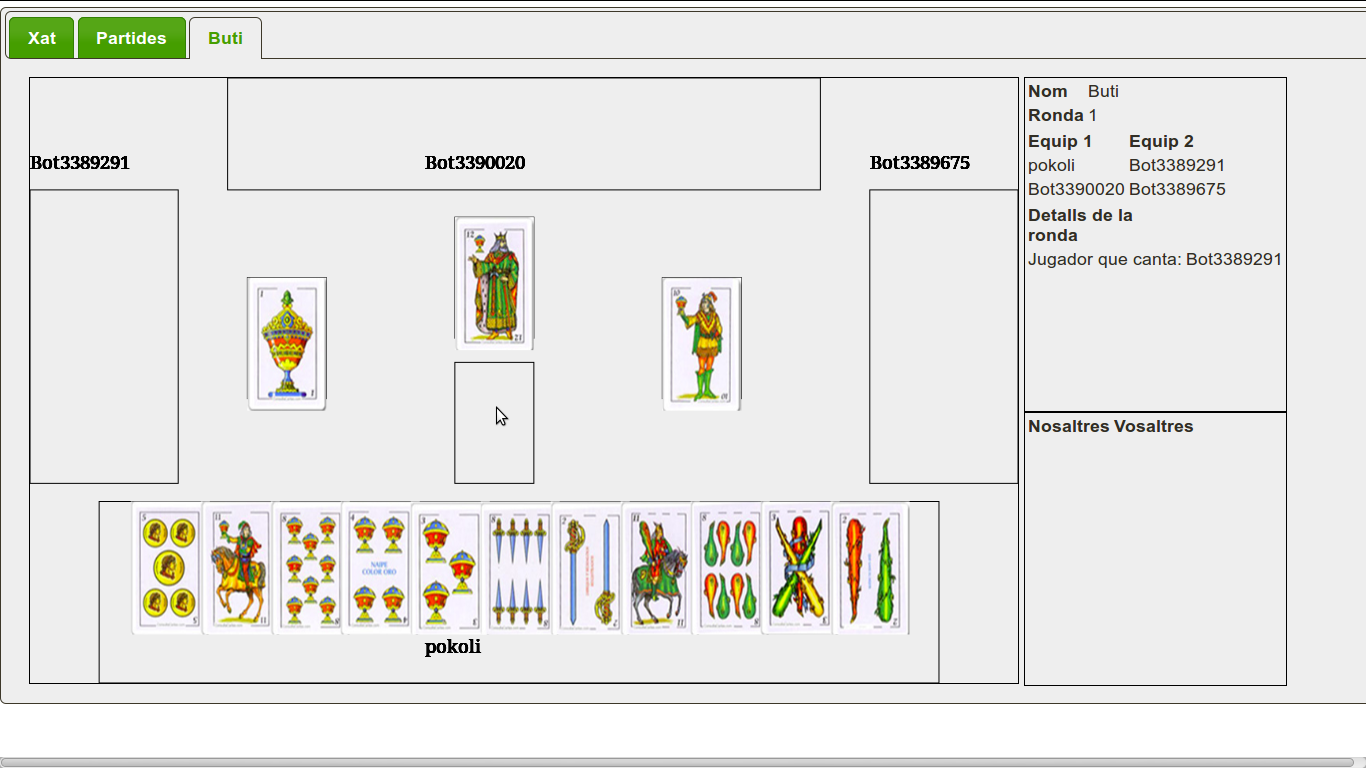
\includegraphics{img/real-partida.png}
\caption{Maqueta de la pantalla de detall de la partida}
\label{fig:real-partida}
\end{figure} 

